\chapter{INTRODUCTION}
\section{Company Profile}
PT. Bank Central Asia Tbk. (BCA) is an Indonesian bank founded on August 10, 1955. But start operating on 21 February 1957. In 1980s, BCA started expanding their branch offices and other services. They also expanded their services to ATM (\textit{Anjungan Tunai Mandiri} or Automated Teller Machine). In 1991, BCA started placing 50 units of ATM in some places in Jakarta.\\

Many things happened since the bank was founded, but the most significant was the Asian financial crisis in 1997. It has tremendous impact on Indonesia's entire banking system, including BCA. In particular, it affected BCA's cash flow and threatened BCA to go bankrupt. It drives BCA to seek assistance from the Indonesian government. Finally the Indonesian Bank Restructuring Agency (IBRA) took over the control of the bank in 1998.\\

At the same year, BCA somehow fully recovered and it's assets stood at Rp 67.93 trillion. Public confidence of BCA was finally restored, and in 2001 they were released by IBRA to BI (Bank Indonesia). In 2000, BCA started become IPO (Initial public Offering) and selling their 22.55\% of their shares that were being divested by IBRA. On secondary public offering which was held on July 2001, BCA offered their 10\% of total shares. Which left them 60.3\% of their own shares. In 2016, BCA's shares are 52.85\% held by public.\\

Until 2016, BCA had more than 15 millions customer in Indonesia. To coordinate their enterprise to reach whole Indonesia, BCA distributed into 12 regions which consist of 135 main branches, 874 sub branches, 222 and cash offices. BCA had hired 25.073 employees in total, which increased by 4.5\% compared in 2015.\\

Company's Vision:
\begin{itemize}
	\itemsep0em
    \item To be the bank of choice and a major pillar of the Indonesian economy
\end{itemize}

Company's Mission:
\begin{itemize}
	\itemsep0em
    \item To build centers of excellence in payment settlements and financial solutions for business and individuals
    \item To understand diverse customer needs and provide the right financial services to optimize customer satisfaction
    \item To enhance our corporate franchise and stakeholders value
\end{itemize}

\section{Student Positions and Roles}
On internship program this odd semester, the author got assigned at Strategic Information Technology Group (GSIT) division, Data Management (DTM) work unit, Datawarehouse (DWH) team. The author was asked to assisting some of other collage's projects, and primary asked to help with data migration.

\begin{figure}[H]
\centering
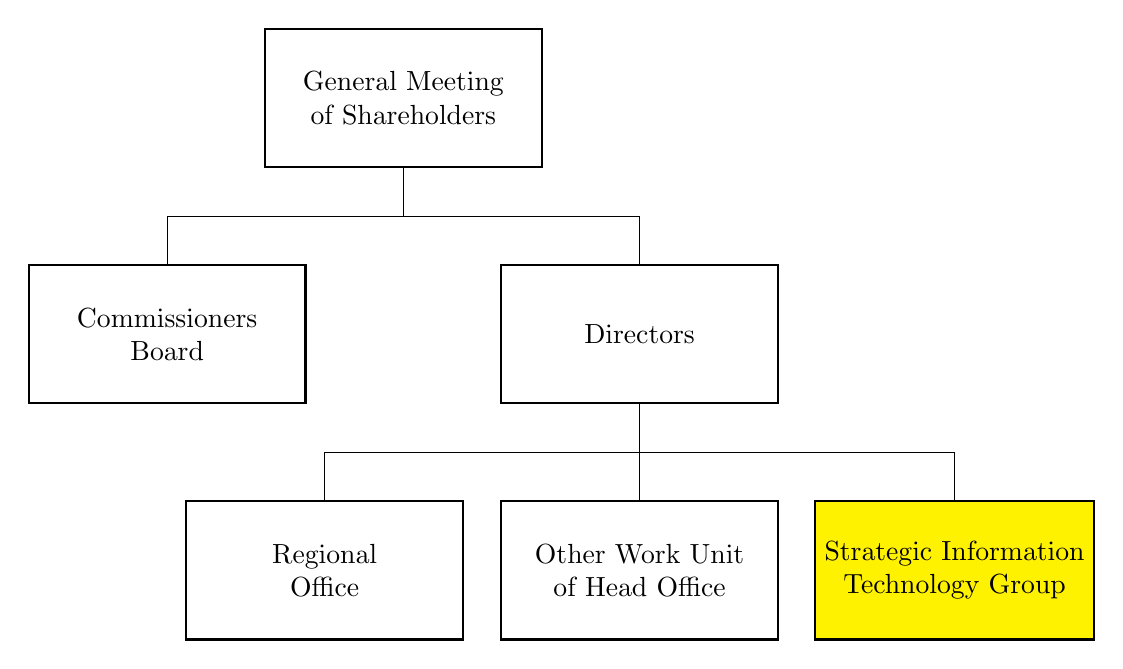
\begin{tikzpicture}
	\tikzset{every node/.style=
        {thick, draw=black, align=center, minimum height=50pt, minimum width=100pt}
     }
	\node (root) at (5,3) [draw] {General Meeting\\of Shareholders};
	\node (l1n1) at (2,0) [draw] {Commissioners\\Board};
	\node (l1n2) at (8,0) [draw] {Directors};
	\node (l2n1) at (4,-3) [draw] {Regional\\Office};
	\node (l2n2) at (8,-3) [draw] {Other Work Unit\\of Head Office};
	\node[fill=yellow] (l2n3) at (12,-3) [draw] {Strategic Information\\Technology Group};
	\draw (node cs:name=l1n1,anchor=north) |- (5,1.5);
	\draw (node cs:name=l1n2,anchor=north)|- (5,1.5) -| (node cs:name=root,anchor=south);
	\draw (node cs:name=l2n1, anchor=north) |- (9,-1.5);
	\draw (node cs:name=l2n2, anchor=north) |- (9,-1.5);
	\draw (node cs:name=l2n3, anchor=north) |- (9,-1.5) -| (node cs:name=l1n2, anchor=south);
\end{tikzpicture}
\caption{BCA's organization structure}
\end{figure}

This year and last year, migration data became the priority in this team. Because the server of ETL old program that were use for ETL jobs were going to be shut down soon. So, the author's daily job was to migrate the jobs of ETL to the new ETL program.

\begin{figure}[H]
\centering
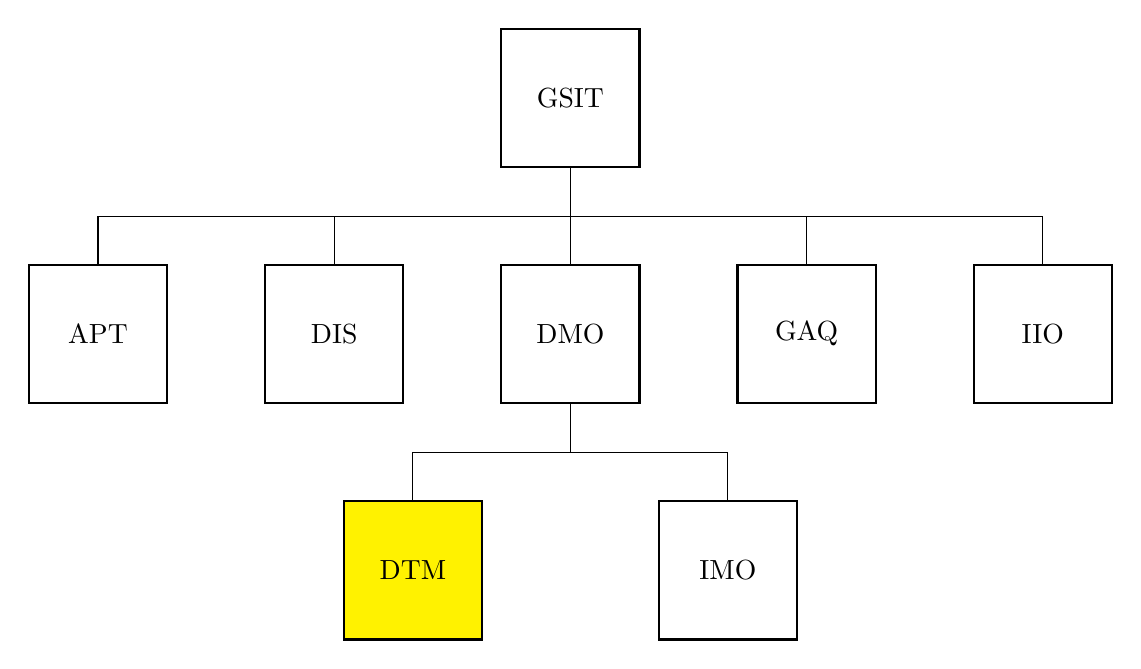
\begin{tikzpicture}
	\tikzset{every node/.style=
        {thick, draw=black, align=center, minimum height=50pt, minimum width=50pt}
     }
	\node (root) at (5,3) [draw] {GSIT};
	\node (l1n1) at (-1,0) [draw] {APT};
	\node (l1n2) at (2,0) [draw] {DIS};
	\node (l1n3) at (5,0) [draw] {DMO};
	\node (l1n4) at (8,0) [draw] {GAQ};
	\node (l1n5) at (11,0) [draw] {IIO};
	\node[fill=yellow] (l2n1) at (3,-3) [draw] {DTM};
	\node (l2n2) at (7,-3) [draw] {IMO};
	
	\draw (node cs:name=l1n1,anchor=north) |- (5,1.5);
	\draw (node cs:name=l1n2,anchor=north) |- (5,1.5);
	\draw (node cs:name=l1n3,anchor=north)|- (5,1.5) -| (node cs:name=root,anchor=south);
	\draw (node cs:name=l1n4,anchor=north) |- (5,1.5);
	\draw (node cs:name=l1n5,anchor=north) |- (5,1.5);
	\draw (node cs:name=l2n1, anchor=north) |- (5,-1.5);
	\draw (node cs:name=l2n2, anchor=north) |- (5,-1.5) -| (node cs:name=l1n3, anchor=south);
\end{tikzpicture}
\caption{GSIT organization structure}
\end{figure}